\chapter{Electrochemical Systems}

A typical electrochemical experiment uses an electrochemical cell to drive
reduction and oxidation (redox) reactions at the surface of a working
electrode. The cell consists of at least two electrodes immersed in an
electrolyte solution: the \emph{working electrode}, at whose surface the
reaction of interest takes place, and a \emph{counter electrode}, which
completes the circuit. A third \emph{reference electrode} is commonly
included to provide a stable, known potential against which the potential
of the working electrode is measured and controlled. A device called a
\emph{potentiostat} maintains the desired potential difference between the
working and reference electrodes, drives the current through the circuit
formed by the working and counter electrodes, and simultaneously measures
that current.

\begin{figure}
  \centering
  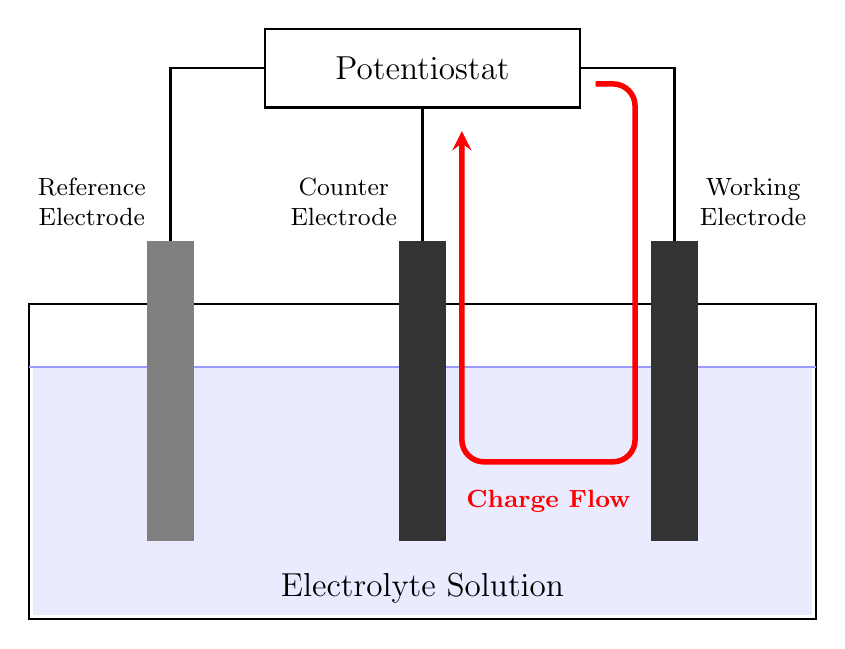
\begin{tikzpicture}[>=stealth, thick]

  % Solution vessel
  \draw[thick] (0, 0) -- (0, 4) -- (10, 4) -- (10, 0) -- cycle;
  % Solution fill
  \fill[blue!8] (0.05, 0.05) rectangle (9.95, 3.2);
  % Solution surface line
  \draw[blue!40, thick] (0, 3.2) -- (10, 3.2);
  \node[font=\large] at (5, 0.4) {Electrolyte Solution};

  % Potentiostat box
  \draw[thick, fill=white] (3, 6.5) rectangle (7, 7.5);
  \node[font=\large] at (5, 7) {Potentiostat};

  % Reference Electrode (left)
  \fill[black!50] (1.5, 1.0) rectangle (2.1, 4.8);
  \node[font=\small, align=center] at (0.8, 5.3) {Reference\\Electrode};
  % Wire from counter electrode to potentiostat
  \draw[thick] (1.8, 4.8) -- (1.8, 7) -- (3, 7);

  % Counter Electrode (centre)
  \fill[black!80] (4.7, 1.0) rectangle (5.3, 4.8);
  \node[font=\small, align=center] at (4.0, 5.3) {Counter\\Electrode};
  % Wire from reference electrode to potentiostat
  \draw[thick] (5.0, 4.8) -- (5.0, 6.5);

  % Working Electrode (right)
  \fill[black!80] (7.9, 1.0) rectangle (8.5, 4.8);
  \node[font=\small, align=center] at (9.2, 5.3) {Working\\Electrode};
  % Wire from working electrode to potentiostat
  \draw[thick] (8.2, 4.8) -- (8.2, 7) -- (7, 7);

  % Charge flow arrows (red loop)
  \draw[->, red, line width=2pt, rounded corners=8pt]
  (7.2, 6.8) -- (7.7, 6.8) -- (7.7, 2.0) -- (5.5, 2.0)
  -- (5.5, 4.0) -- (5.5, 6.2);
  \node[red, font=\small\bfseries] at (6.6, 1.5) {Charge Flow};

\end{tikzpicture}

  \caption{Schematic of a three-electrode electrochemical cell. The
    potentiostat controls the potential difference between the working
    and reference electrodes whilst driving current (red) through the
    circuit formed by the working and counter electrodes via the
  analyte solution.}
  \label{fig:electrochemical-cell}
\end{figure}

The reaction occurring at the working electrode surface depends on the
applied potential and the chemical species present in solution. In the
simplest case, a solution-phase species undergoes a single-electron redox
reaction:
\begin{equation}\label{eq:redox}
  \mathrm{A} + \mathrm{e}^{-} \rightleftharpoons \mathrm{B},
\end{equation}
where species $\mathrm{A}$ is reduced --- that is, it gains one electron ---
to form species $\mathrm{B}$. The reverse process, in which $\mathrm{B}$
loses an electron to regenerate $\mathrm{A}$, is the corresponding
oxidation. Throughout this chapter we restrict attention to this
single-electron ($n = 1$) process and adopt the convention that a
\emph{positive} current corresponds to net reduction (cathodic current).

\section{Voltammetry}

Voltammetry is the class of electroanalytical techniques in which the
potential applied to the working electrode is varied in a prescribed
manner and the resulting current is recorded. Because the current is
directly related to the rate of the electrochemical reaction at the
electrode surface, the current--potential curve --- called a
\emph{voltammogram} --- encodes information about the kinetics of the
redox process as well as the transport of chemical species in solution.

In a cyclic voltammetry (CV) experiment the applied potential is swept
linearly with time from a starting potential~$E_i$, chosen so that the
overpotential is insufficient to drive any significant reaction, towards
more negative values (for a reduction) until a vertex potential~$E_v$ is
reached. The vertex potential is chosen sufficiently beyond the formal
potential of the redox couple that the reaction is driven to completion at
the electrode surface; it serves only as the turning point of the sweep.
The potential is then swept back to~$E_i$, reversing the direction of
electron transfer and reforming~$\mathrm{A}$. This triangular waveform is
illustrated in the left panel of \cref{fig:potential-voltammagram}.

Throughout this process the current $I$ is recorded. Plotting the current
against the applied potential gives the voltammogram shown in the right
panel of \cref{fig:potential-voltammagram}. The forward sweep produces
a reduction (cathodic) peak as the potential moves through the range at
which $\mathrm{A}$ is converted to $\mathrm{B}$; the return sweep produces
an oxidation (anodic) peak as $\mathrm{B}$ is reconverted to $\mathrm{A}$.

The peak shape arises from competition between two rate-limiting
processes. During the early part of the forward sweep the applied
potential is positive relative to the formal potential of the redox
couple, so there is insufficient driving force to reduce $\mathrm{A}$ and
negligible current flows. As the potential is swept to more negative
values the reduction reaction becomes progressively more
thermodynamically favourable and the current increases: during this rising
portion the system is under \emph{kinetic control}, meaning that the rate
of electron transfer at the electrode surface is the rate-limiting step.
Eventually the concentration of~$\mathrm{A}$ in the immediate vicinity of
the electrode is depleted to near zero and the current reaches a peak.
Beyond this point the current decays despite the continued increase in
thermodynamic driving force, because the reaction has passed into
\emph{diffusional control}: the rate at which fresh~$\mathrm{A}$ can be
transported to the electrode by diffusion is now the limiting factor.

\begin{figure}
  \begin{center}
    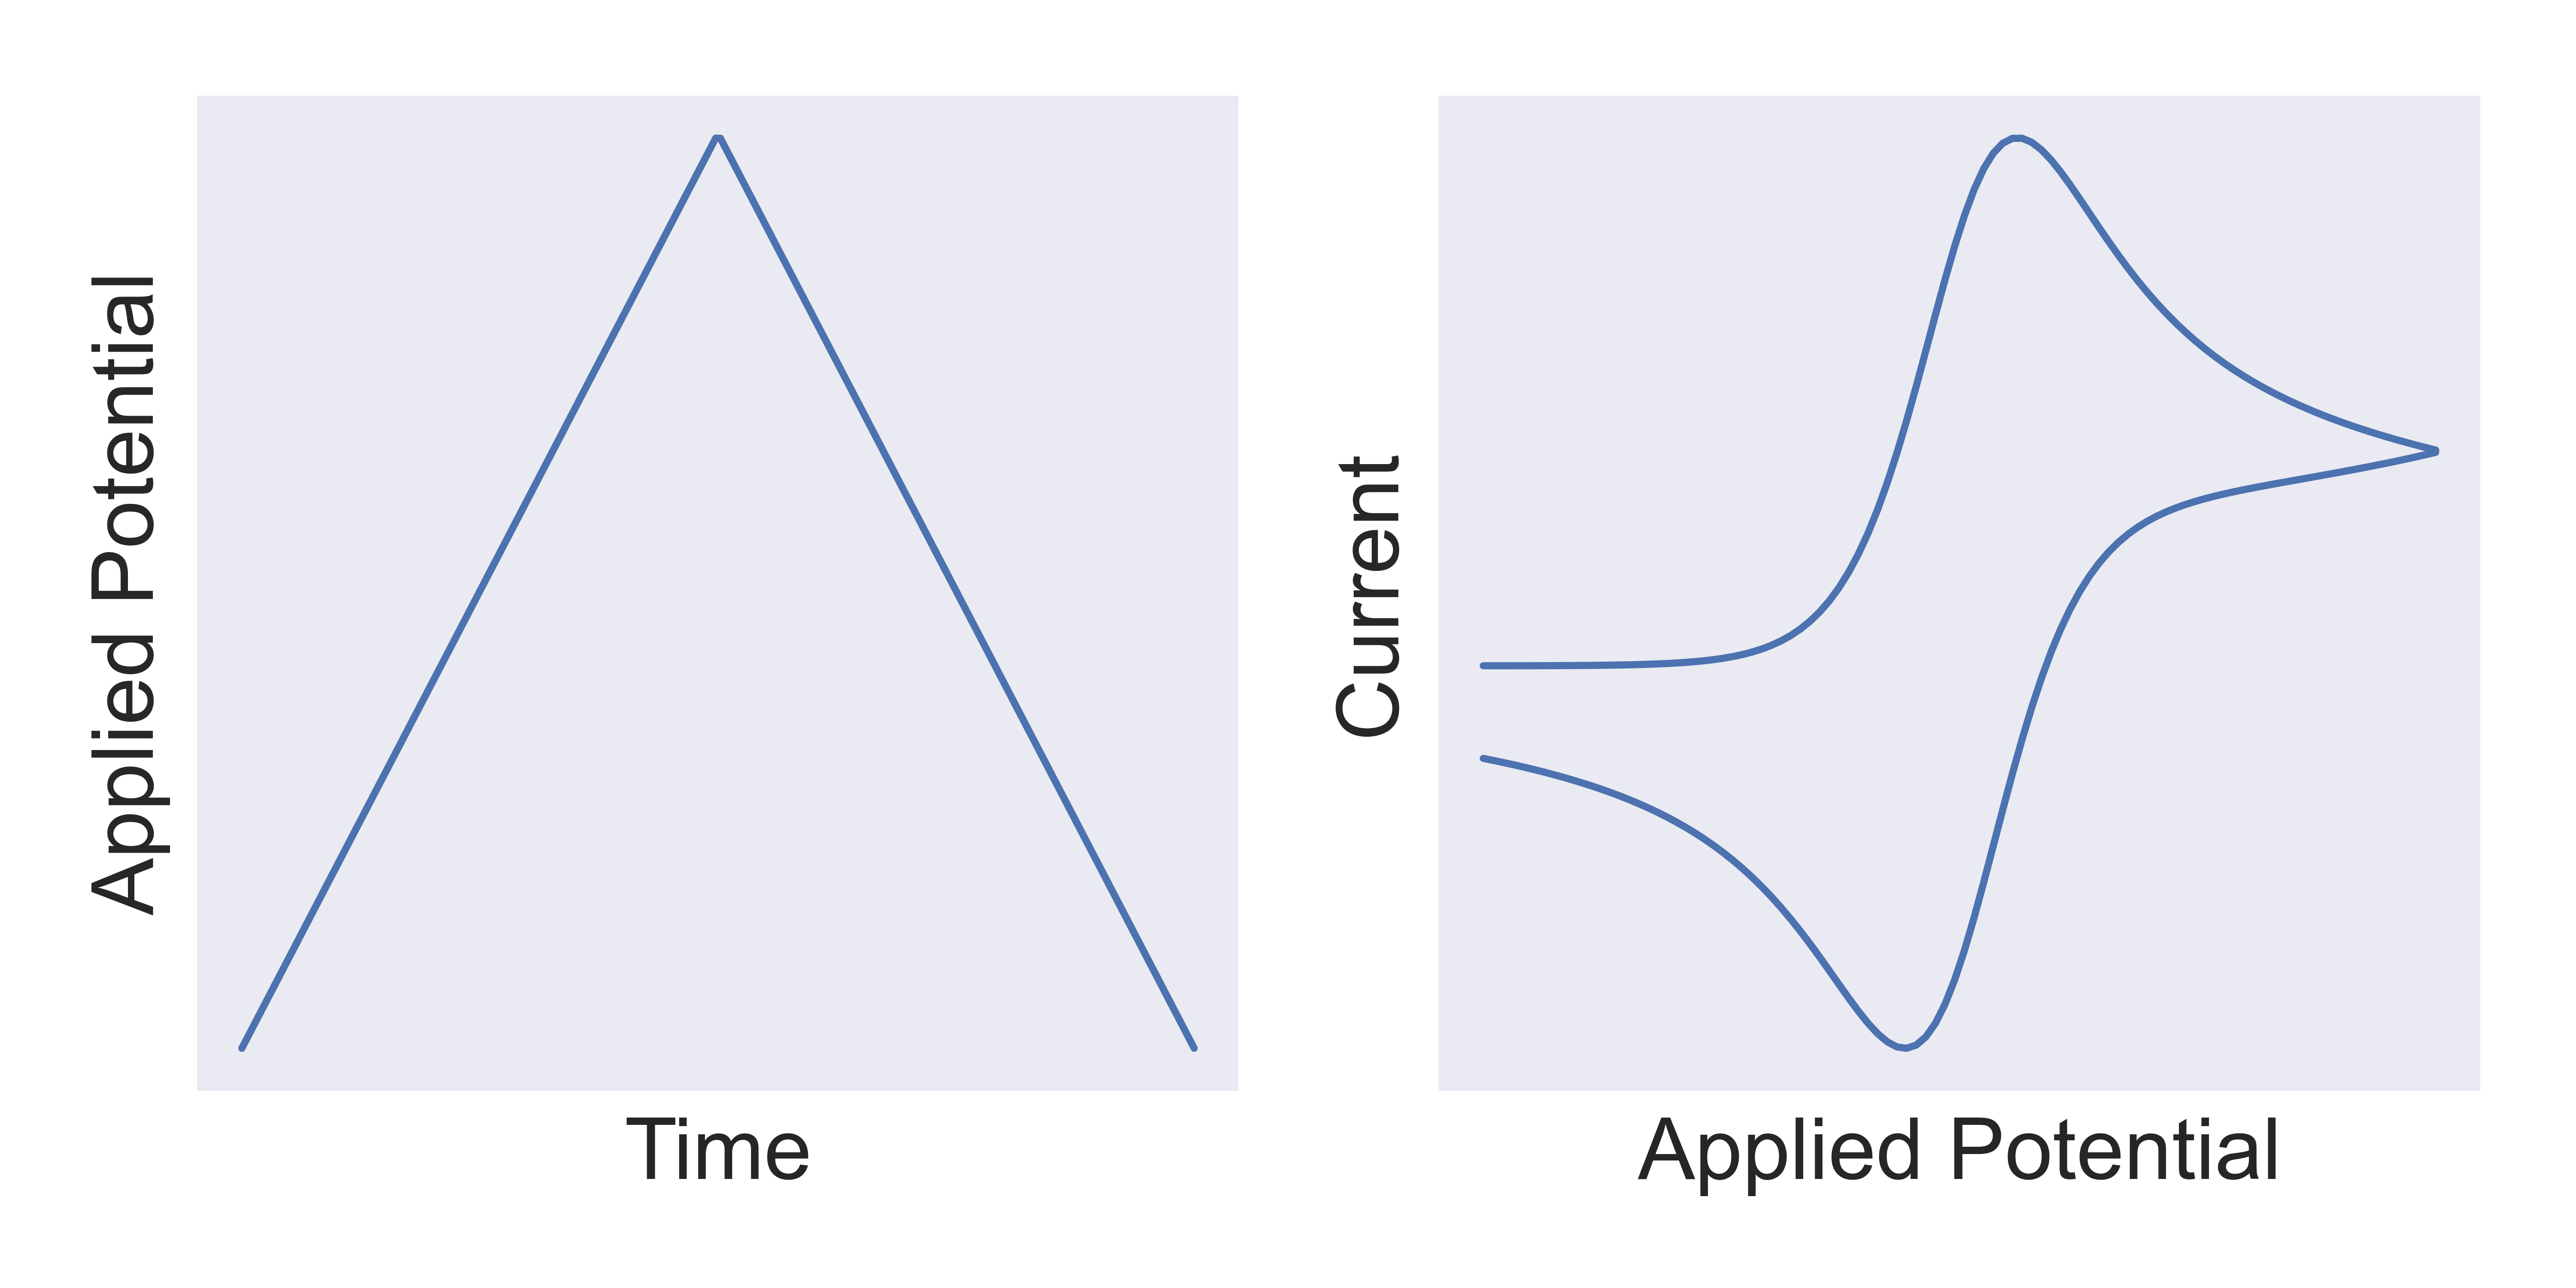
\includegraphics[width=0.8\textwidth]{figures/applied-potential-and-voltammagram.png}
  \end{center}
  \caption[Applied potential and voltammogram example]{Left: the triangular
    potential waveform applied in a cyclic voltammetry experiment. Right:
    the resulting reversible reaction's voltammogram showing the cathodic
    (reduction) peak which occurs on the forward sweep and the anodic
  (oxidation) peak which occurs on the reverse sweep.}
  \label{fig:potential-voltammagram}
\end{figure}

Cyclic Voltammetry is particularly useful because the position, shape, and
relative heights of the peaks provide a signature of the
electrochemical process. The potential at which each peak occurs is related
to the formal potential $E^{\circ}_f$, and the separation between
the cathodic and anodic peaks carries information about the electrode
kinetics, as discussed in \cref{sec:electrode-kinetics}.

The \emph{scan rate} $\nu$ $(\mathrm{V\,s^{-1}})$ is the constant rate at
which the potential is swept, defined as
\begin{equation}
  \nu = \frac{dE}{dt}.
  \label{eq:scan_rate}
\end{equation}
The scan rate is an important experimental parameter: faster scans probe
shorter timescales and can resolve kinetic processes that would otherwise
reach equilibrium on a slower scan, whilst slower scans allow more time for
diffusion and can reveal coupled chemical reactions.

\section{Mathematical Description}

We now formulate the governing equations for the system. The first
assumption we make is that we have a ``macro''-electrode: specifically, we
consider a planar disc electrode of radius~$\epsilon$, whose characteristic
dimension is much larger than the distance over which species can diffuse
on the timescale of the experiment. As a consequence, edge effects are
negligible and we can model only the diffusion perpendicular to the
electrode surface, reducing the problem to one spatial dimension.

\begin{figure}
  \centering
  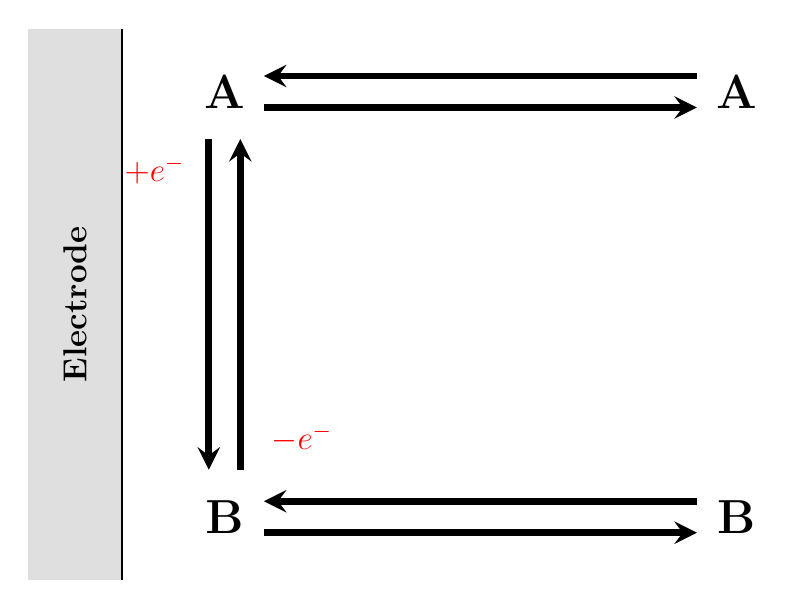
\begin{tikzpicture}[>=stealth, thick]
  % Electrode block
  \fill[gray!25] (-1.2, -1) rectangle (0, 6);
  \draw[thick] (0, -1) -- (0, 6);
  \node[rotate=90, font=\large\bfseries] at (-0.6, 2.5) {Electrode};
  % Species A row (top)
  \node[font=\LARGE\bfseries] at (1.3, 5.2) {A};
  \node[font=\LARGE\bfseries] at (7.8, 5.2) {A};
  % A: arrows
  \draw[->, line width=2.5pt] (7.3, 5.4) -- (1.8, 5.4);
  \draw[->, line width=2.5pt] (1.8, 5.0) -- (7.3, 5.0);
  % Species B row (bottom)
  \node[font=\LARGE\bfseries] at (1.3, -0.2) {B};
  \node[font=\LARGE\bfseries] at (7.8, -0.2) {B};
  % B: arrows
  \draw[->, line width=2.5pt] (7.3, 0.0) -- (1.8, 0.0);
  \draw[->, line width=2.5pt] (1.8, -0.4) -- (7.3, -0.4);
  % Electron transfer arrows
  \draw[->, line width=2.5pt] (1.1, 4.6) -- (1.1, 0.4);
  \node[left, font=\large] at (2.8, 0.8) {\textcolor{red}{$-e^-$}};
  \draw[->, line width=2.5pt] (1.5, 0.4) -- (1.5, 4.6);
  \node[right, font=\large] at (-0.1, 4.2) {\textcolor{red}{$+e^-$}};
\end{tikzpicture}

  \caption{Schematic of the one-dimensional electrode reaction. Species
    $\mathrm{A}$ diffuses from the bulk solution towards the electrode
    surface, where it is reduced ($+e^-$) to form species $\mathrm{B}$.
    The reverse oxidation ($-e^-$) converts $\mathrm{B}$ back to
    $\mathrm{A}$. Species $\mathrm{B}$ diffuses away from the electrode
  into the bulk.}
\end{figure}

\subsection{Diffusion: Fick's Second Law}\label{sec:diffusion}

We model the transport of species in quiescent (unstirred) solution using
Fick's second law~\cite{crank1979mathematics}, which describes the
evolution of a concentration field $c(x,t)$ due to diffusion. For the
couple $\mathrm{A}/\mathrm{B}$ on the planar
electrode we have the system
\begin{equation}
  \begin{aligned}
    \frac{\partial c_A}{\partial t}
    &= D_A \frac{\partial^2 c_A}{\partial x^2}, \\
    \frac{\partial c_B}{\partial t}
    &= D_B \frac{\partial^2 c_B}{\partial x^2},
  \end{aligned}
  \label{eq:diffusion}
\end{equation}
where $D_A$ and $D_B$ $(\mathrm{m^2\,s^{-1}})$ are the diffusion
coefficients of the respective species and $x$ denotes the distance from
the electrode surface. Each equation is a linear parabolic partial
differential equation defined on the semi-infinite domain $x \geq 0$.

\subsection{Fick's First Law and Electrode
Kinetics}\label{sec:electrode-kinetics}

Fick's first law~\cite{crank1979mathematics} states that the diffusive
flux through a plane normal to the $x$-axis at a point $x^*$ is
proportional to the concentration gradient at that point:
\begin{equation}
  j_{x^*} = -D\left(\frac{\partial c}{\partial x}\right)\bigg|_{x = x^*},
  \label{eq:ficks-first}
\end{equation}
where the negative sign indicates that the flux is directed down the
concentration gradient.

The rate at which the electrode reaction~\cref{eq:redox} proceeds is
governed by the applied potential. The standard model for electrode
kinetics is the Butler--Volmer equation~\cite{dickinson2020butler}, which
relates the applied potential $E(t)$ to the net flux of $\mathrm{A}$ at
the electrode surface:
\begin{equation}
  j_{0, A} = k_0 \left[ c_A(t,0)\,
    e^{-\alpha \frac{F}{\mathcal{R}\mathcal{T}} (E(t) - E^0_f)}
    - c_B(t,0)\,
    e^{(1-\alpha) \frac{F}{\mathcal{R}\mathcal{T}} (E(t) - E^0_f)}
  \right],
  \label{eq:butler-volmer}
\end{equation}
where $k_0$ $(\mathrm{m\,s^{-1}})$ is the standard rate constant, $\alpha
\in (0,1)$ is the transfer coefficient, $F$ is Faraday's constant,
$\mathcal{R}$ is the
universal gas constant, and $\mathcal{T}$ is the absolute temperature.
The quantity $E(t) - E^0_f$ is the overpotential, measuring the
deviation of the applied potential from the formal potential. The first
exponential term represents the reduction contribution: a negative
overpotential ($E(t) < E^0_f$) enhances this term and drives the
conversion of $\mathrm{A}$ to $\mathrm{B}$. The second exponential
represents the oxidation contribution, which dominates when the
overpotential is positive. In the limit of large $k_0$ the exponential
terms force the surface concentrations towards thermodynamic equilibrium
and the system exhibits reversible behaviour; when $k_0$ is small the
reaction is kinetically limited and the flux is directly proportional
to~$k_0$, giving irreversible behaviour.

Combining \cref{eq:ficks-first,eq:butler-volmer} at the electrode surface
($x = 0$) yields a Neumann boundary condition for the diffusion
equations:
\begin{equation}
  -D_A\left(\frac{\partial c_A}{\partial x}\right)\bigg|_{x = 0} =
  k_0 \left[ c_A(t,0)\,
    e^{-\alpha \frac{F}{\mathcal{R}\mathcal{T}} (E(t) - E^0_f)}
    - c_B(t,0)\,
    e^{(1-\alpha) \frac{F}{\mathcal{R}\mathcal{T}} (E(t) - E^0_f)}
  \right].
  \label{eq:electrode-boundary-condition}
\end{equation}
Conservation of mass at the electrode surface requires that whatever is
consumed of $\mathrm{A}$ is produced as $\mathrm{B}$, and vice versa. Since
we consider a single-electron process with no homogeneous reactions in
solution, this is simply stoichiometric conservation:
\begin{equation}
  D_B\left(\frac{\partial c_B}{\partial x}\right)\bigg|_{x = 0} =
  -D_A\left(\frac{\partial c_A}{\partial x}\right)\bigg|_{x = 0}.
  \label{eq:mass-conservation}
\end{equation}

\subsection{Boundary and Initial Conditions}

At the start of the experiment we assume that $\mathrm{A}$ is at some
bulk concentration $c_A^*$ and that $\mathrm{B}$ is at bulk concentration
$c_B^*$:
\begin{equation}
  \begin{aligned}
    c_A(0, x) &= c_A^*, \\
    c_B(0, x) &= c_B^*.
  \end{aligned}
  \label{eq:initial-conditions}
\end{equation}
Far from the electrode surface, the redox reaction has no effect on the
concentrations, so the bulk values are recovered:
\begin{equation}
  \begin{aligned}
    c_A(t, x) &\to c_A^* \quad \text{as } x \to \infty, \\
    c_B(t, x) &\to c_B^* \quad \text{as } x \to \infty.
  \end{aligned}
  \label{eq:infinite-boundary-condition}
\end{equation}

\subsection{Current}

The primary experimental observable of a voltammetry experiment is the
current measured by the potentiostat. At any instant the current for the
single-electron reduction of species $\mathrm{A}$ is
\begin{equation}
  I = F A_{\mathrm{el}}\, j_{0, A},
  \label{eq:current}
\end{equation}
where $A_{\mathrm{el}} = \pi\epsilon^2$ is the area of the disc electrode
and $j_{0, A}$ is the net flux of species $\mathrm{A}$ at the electrode
surface, which is proportional to the concentration gradient at that point
by Fick's first law~\cref{eq:ficks-first}. Under our sign convention a
positive $j_{0,A}$ corresponds to net consumption of~$\mathrm{A}$ at the
surface (reduction) and hence a positive current. Computing the current
therefore reduces to evaluating how $j_{0, A}$ evolves in time.

\section{Non-Dimensionalisation}

The combination of
\cref{eq:diffusion,eq:electrode-boundary-condition,eq:mass-conservation,%
eq:initial-conditions,eq:infinite-boundary-condition} constitutes an
initial-boundary value problem. It is advantageous to solve a
non-dimensional version of this problem: the results of a single
non-dimensional simulation can be rescaled to any combination of physical
parameters without rerunning the computation. We non-dimensionalise in the
standard way, scaling concentrations by the bulk concentration
of~$\mathrm{A}$, diffusion coefficients by~$D_A$, lengths by the
electrode radius~$\epsilon$, and potentials by the thermal voltage
$\mathcal{R}\mathcal{T}/F$.

We present a summary of the normalisation in \cref{tab:normalisation}.

\begin{table}[ht]
  \centering
  \begin{tabular}{ll}
    \hline
    Parameter & Normalisation \\
    \hline
    concentration & $C_j = c_j / c_{\mathrm{A}}^*$ \\
    diffusion coefficient & $d_j = D_j / D_{\mathrm{A}}$ \\
    spatial coordinate & $X = x / \epsilon$ \\
    time & $T = D_{\mathrm{A}} t / \epsilon^2$ \\
    applied potential & $\theta = (F / \mathcal{R}\mathcal{T})\,E$ \\
    formal potential & $\theta_f = (F /
    \mathcal{R}\mathcal{T})\,E_{\mathrm{f}}^0$ \\
    rate constant & $K_0 = k_0\,\epsilon / D_{\mathrm{A}}$ \\
    scan rate & $\sigma = (\epsilon^2 / D_{\mathrm{A}})(F /
    \mathcal{R}\mathcal{T})\,\nu$ \\
    current & $J = I / (\pi \epsilon F D_{\mathrm{A}} c_{\mathrm{A}}^*)$ \\
    \hline
  \end{tabular}
  \caption{Dimensionless normalisation of variables. Here $\epsilon$ is the
  radius of the disc electrode.}
  \label{tab:normalisation}
\end{table}

We define the dimensionless concentration, diffusion coefficient, spatial
coordinate, and time as
\begin{equation}
  C_j = \frac{c_j}{c_A^*}, \quad d_j = \frac{D_j}{D_A}, \quad X =
  \frac{x}{\epsilon}, \quad T = \frac{D_A\, t}{\epsilon^2},
  \label{eq:nd_CdXT}
\end{equation}
and the dimensionless rate constant as
\begin{equation}
  K_0 = \frac{k_0\,\epsilon}{D_A}.
  \label{eq:nd_K0}
\end{equation}
We now substitute these into the governing equations, initial conditions,
and boundary conditions.

\subsection{Governing Equation}

Considering the left-hand side of \cref{eq:diffusion}:
$$
\frac{\partial c_j}{\partial t}
= \frac{\partial c_j}{\partial C_j}\frac{\partial C_j}{\partial t}
= c_A^*\frac{\partial C_j}{\partial t}
= \frac{c_A^* D_A}{\epsilon^2}\frac{\partial C_j}{\partial T}.
$$
Now the right-hand side:
$$
D_j \frac{\partial^2 c_j}{\partial x^2}
= D_j \frac{c_A^*}{\epsilon^2}\frac{\partial^2 C_j}{\partial X^2}
= d_j \frac{c_A^* D_A}{\epsilon^2}\frac{\partial^2 C_j}{\partial X^2}.
$$
Equating gives the dimensionless diffusion equation:
\begin{equation}
  \frac{\partial C_j}{\partial T} = d_j \frac{\partial^2 C_j}{\partial X^2}.
  \label{eq:nd_diffusion}
\end{equation}

\subsection{Initial and Far-Field Conditions}

The initial conditions become
\begin{equation}
  \begin{aligned}
    C_A(0, X) &= 1, \\
    C_B(0, X) &= C_B^*.
  \end{aligned}
  \label{eq:nondim_initial_conditions}
\end{equation}

In practice we cannot simulate a semi-infinite domain. Einstein's analysis
of Brownian motion~\cite{einstein1905brownian} shows that the root-mean-square
displacement of a diffusing particle is $x_{\mathrm{rms}} = \sqrt{2Dt}$.
To ensure the outer boundary is sufficiently remote that it is unaffected
by diffusion, we truncate the domain at $X_{\mathrm{max}} =
6\sqrt{T_{\mathrm{sim}}}$
in dimensionless form. The far-field boundary conditions are then
\begin{equation}
  \begin{aligned}
    C_A(T,\, X_{\mathrm{max}}) &= 1, \\
    C_B(T,\, X_{\mathrm{max}}) &= C_B^*.
  \end{aligned}
  \label{eq:nd_far_field}
\end{equation}

\subsection{Electrode Surface Boundary}

We define the dimensionless applied and formal potentials as
\begin{equation}
  \begin{aligned}
    \theta(T) &= \frac{F}{\mathcal{R}\mathcal{T}}\, E(t), \\
    \theta_f &= \frac{F}{\mathcal{R}\mathcal{T}}\, E^0_f.
  \end{aligned}
  \label{eq:nondim-potentials}
\end{equation}
Substituting the dimensionless variables into
\cref{eq:electrode-boundary-condition,eq:mass-conservation} and using the
definition of~$K_0$ from \cref{eq:nd_K0}, the Butler--Volmer boundary
condition and the mass conservation condition become
\begin{equation}
  \begin{aligned}
    \frac{\partial C_A}{\partial X}\bigg|_{X=0} &=
    K_0 \left[ C_A(T,0)\, e^{-\alpha(\theta(T) - \theta_f)}
    - C_B(T,0)\, e^{(1-\alpha)(\theta(T) - \theta_f)} \right], \\
    d_B \frac{\partial C_B}{\partial X}\bigg|_{X=0} &=
    -\frac{\partial C_A}{\partial X}\bigg|_{X=0}.
  \end{aligned}
  \label{eq:nondim-electrode-boundary}
\end{equation}

\subsection{Scan Rate}

As defined in \cref{eq:scan_rate}, the scan rate is the rate of change of
potential with respect to time. We therefore define a dimensionless scan
rate $\sigma$ as the rate of change of dimensionless potential with
respect to dimensionless time:
\begin{equation}
  \sigma = \frac{d\theta}{dT}.
  \label{eq:nd_scan_rate}
\end{equation}
To relate $\sigma$ to $\nu$ we note that
$$
\nu = \frac{\partial E}{\partial t}
= \frac{\mathcal{R}\mathcal{T}}{F}\frac{\partial \theta}{\partial t}
= \frac{\mathcal{R}\mathcal{T} D_A}{F \epsilon^2}\frac{\partial
\theta}{\partial T},
$$
and hence
\begin{equation}
  \sigma = \frac{F \epsilon^2}{\mathcal{R}\mathcal{T} D_A}\, \nu.
  \label{eq:sigma_nu}
\end{equation}

\subsection{Current}

Since the model is now in dimensionless units we cannot compute the flux
$j_{0,A}$ directly, but we can compute a dimensionless flux and relate the
two. We define
\begin{equation}
  J_{X^*,\, j} = -d_j \left(\frac{\partial C_j}{\partial X}\right)_{X^*}.
  \label{eq:nd_flux}
\end{equation}
To recover the dimensional flux, we note that
$$
j_j = -D_j \left(\frac{\partial c_j}{\partial x}\right)_{x^*}
= -d_j \frac{c_A^* D_A}{\epsilon}\frac{\partial C_j}{\partial X}
= \frac{c_A^* D_A}{\epsilon}\, J_j.
$$
Substituting into \cref{eq:current} with $A_{\mathrm{el}} = \pi\epsilon^2$
gives
\begin{equation}
  I = \pi \epsilon\, F\, D_A\, c_A^*\, J_{0,A}.
  \label{eq:nondim_current}
\end{equation}
When we run a simulation we record the dimensionless flux $J$ as a
function of the dimensionless potential $\theta$. To obtain the physical
voltammogram the results need only be scaled by the values of $c_A^*$,
$D_A$, and $\epsilon$. Consequently, the results of a single simulation
apply to any set of these parameters; the simulation does not need to be
rerun when, for example, the bulk concentration of $\mathrm{A}$ is
changed.

\section{Equal Diffusion Coefficients}

For the remainder of this dissertation we assume that all diffusion
coefficients are equal, i.e.\ $d_B = 1$. This assumption allows us to
solve for the concentration of $\mathrm{A}$ alone and infer the
concentration of $\mathrm{B}$.

From the mass conservation condition~\cref{eq:nondim-electrode-boundary}, when
$d_B = 1$ the surface flux condition simplifies to
\begin{equation}
  \frac{\partial C_B}{\partial X}\bigg|_{X=0}
  = -\frac{\partial C_A}{\partial X}\bigg|_{X=0}.
  \label{eq:equal_diff_surface}
\end{equation}
Since the diffusion coefficients are equal and both species satisfy the
same diffusion equation, the sum $C_A + C_B$ satisfies
\begin{equation}
  \frac{\partial(C_A + C_B)}{\partial T}
  = \frac{\partial^2(C_A + C_B)}{\partial X^2}
\end{equation}
with homogeneous Neumann conditions at $X = 0$ (by
\cref{eq:equal_diff_surface}) and constant far-field values. Together with
the initial conditions, this implies that $C_A + C_B$ is constant
everywhere in space and time. Any decrease in $C_A$ is therefore matched
by an equal increase in $C_B$, and vice versa, so that
\begin{equation}
  C_A + C_B = 1 + C_B^*.
\end{equation}
We henceforth drop the subscript and write $C \equiv C_A$, with
$C_B = 1 + C_B^* - C$. The electrode boundary condition then reduces to
\begin{equation}
  \frac{\partial C}{\partial X}\bigg|_{X=0} =
  K_0 \left[ C(T,0)\, e^{-\alpha(\theta(T) - \theta_f)}
  - (1 + C_B^* - C(T,0))\, e^{(1-\alpha)(\theta(T) - \theta_f)} \right].
  \label{eq:equal_diff_bc}
\end{equation}

For ease of notation we denote:
\begin{equation}
  \begin{aligned}
    K_{\text{red}} &= K_0 \exp\bigg[-\alpha(\theta(T) - \theta_f)\bigg], \\
    K_{\text{ox}} &= K_0 \exp\bigg[(1-\alpha)(\theta(T) - \theta_f)\bigg].
  \end{aligned}
  \label{eq:kred_kox}
\end{equation}
These shorthand expressions are used extensively in the numerical
discretisation that follows in next chapter.
